\section{Our Approach}
\label{sec:approach}
\cut{%%%%%%%%%%%
Our approach should be outlined in the following points:
\begin{enumerate}
\item naive (key) idea: distance covered is (roughly) proportional to time.
Illustrate this using a figure.
\item contacts used to rectify our inference - an (forward-backward)
iterative approach (discuss briefly only).
\item speed distribution to allow variance (Markov random process). 
\item dimension reduction (from 2d to 1d).
\end{enumerate}
}%%%%%%%%%%%%

%In original TIP problem, we have map \textit{M}, a set of moving nodes N, their speeds {v}, their initial locations {li}, and a contact history H. The goal is to find the traces of N which can induce the contacts H.
%In our approach, we need a list of contacts, each one is a 
%bi-gram vector <ID,TIME>. The ID is the person's ID who you meet with. \texttt{TIME} is when you meet him, a map and start, end location. Besides that, we need speed distributions for the person using our system. Compared with the constant speed, a speed distribution is more reasonable.
%

\begin{figure}[th]
\centering
\includegraphics[scale=0.45]{circles.eps}
\caption{Location Inference due to a Contact Event}
\label{fig:circles}
\end{figure}

Figure \ref{fig:circles} illustrates the basic idea of our approach.
Given their initial locations, if $A$ and $B$ move with 
bounded speed in an arbitrary fashion, the maximum areas reachable are
characterized by the two colored circles. If $A$ and $B$ meet at time $t$
and generate a contact, then they are likely to be in the common shaded area
at $t$. This area is usually smaller than the original circles and 
hence limits the possible locations of $A$ and $B$ at $t$. 
If $A$ meets another object $C$ later, then we can treat the shaded area 
as the new ``initial location'' for $A$ at time $t$. The inference
goes on as more contacts of $A$ are considered. 
In a nutshell, the contacts serve to constrain the possible locations 
of the objects, and if objects can only 
move along the paths or roads in the map, then their possible locations are
further constrained (e.g., to highlighted path in Figure \ref{fig:circles}). 

%With a start location, the most common method is to draw a circle 
%centered at the start location. The covered area show the possible 
%location that the person may be. As the time went on, the circle will be larger and larger. But this is barely a localization technique. Since we can never tell where the person is. He is at somewhere within the circle, but we never know that.
%
%When considerate a contact event A meets B at time t, the two circles must have some overlap area. Since that contact record means at time t, the A and B are close to each other. Then, the possible area is change from a circle to a overlap area which is smaller. Contact by contact, the possible area will be smaller and smaller. Finally the remaining location will be accurate enough. But it's not enough. This approach does not include a map. It needs to discrete a 2-dimension world, which makes the calculation costs up. Adding a map can solve this problem. Assume people only moving on roads of a map. This can reduce the complexity significantly. Roads on map can be modeled into a 1-dimension array. This is how we take advantage of social context to infer location, and this approach is what we used in our previous paper\cite{wang2011automatic}. 
%

%So far, we take the advantage of social context. But the speed restriction is too strong to be realistic. So, we propose a new approach, to break this constant speed restriction. The constant speed model gives us one exact result, correct or not, no more candidates. That makes it hard to refine the result through a iterative process. So, rather than infer an exact location, this approach gives a location probability matrix as a inferred result. A speed distribution is needed for location probability computation. 
When each object moves at a speed that follows a probability distribution,
the location of an object at each time point is also probabilistic. Since
the movement can be viewed as a Markov process, location at a time point only
depends on the state (i.e. location probability distribution) at the 
previous time point. Let $L_t^A$ be $A$'s location probablity distribution
over all locations on the map at time $t$, i.e. $L_t^A$ is a vector.
Then
\begin{equation}
\label{eqn:trans}
L_t^A = P \cdot (L_{t-1}^A)^T 
\end{equation}
where $P$ is a transition matrix, and $P_{ij}$ is the probability of $A$ 
moving from location $i$ to location $j$ within a unit time. 
$P_{ij}$ is calculated from $A$'s speed distribution, $S_A$.

%The problem has the \texttt{Markov Random Process} feature, location at present state is independent of location of future and the past. It only depends on the very previous state. For example, at time ${ t }_{ i }$ you are at location ${l}_{x}$, we know that in the next coming 1 second, you will move 1 meter. You may go to location ${l}_{x-1}$ or location ${l}_{x+1}$ at time ${t}_{i+1}$. So, we can guess the location at time ${t}_{i+1}$ only based on it's location at time ${t}_{i}$, no needs it's past or future location information.
%The \texttt{state} here describe the location probability of a person at a certain time. So, each time unit is one state. 


%The speed distribution decides the transition from one state to another. 
%We can get the person's moving distance in unit time by multiply the distribution by unit time length. Suppose that for person $h$ at time $t_i$. $l$ is the road model where $h$ might be at that time. $ {l}_{i}\in l_{t_{i}}$ is the probability of H show up at that location at time $t_{i}$. $L = \begin{pmatrix} l_ {  0}  &l_{1}  &l_{2} &\dots &l_{m} \end{pmatrix} $ The speed distribution of H is S, $ S = \left( \begin{matrix} p_{ s_0 } & p_{s_ 1 } &p_ {s_1 } & \dots  &p_ {s_{ max} } \end{matrix} \right)$. $U_t$ is the unit time.

%So, the transition matrix will be : 
%\[ M = \begin{bmatrix} p_{ s_{ 0 } } & p_{ s_{ 1 } } & p_{ s_{ 2 } } & \dots  & p_{ s_{ max } } & 0 & \dots  & 0 \\ p_{ s_{ 1 } } & p_{ s_{ 0 } } & p_{ s_{ 1 } } & p_{ s_{ 2 } } & \dots  & p_{ s_{ max } } & \dots  & 0 \\ \vdots  & \vdots  &\vdots   & \vdots  & \vdots  & \vdots  &\vdots   & \vdots  \\ 0 & \dots  & p_{ s_{ max } } & \dots  & p_{ s_{ 3 } } & p_{ s_{ 2 } } & p_{ s_{ 1 } } & p_{ s_{ 0 } } \end{bmatrix} \]

%\begin{equation} L_{i+1} = U_t\cdot M \cdot L_{i}\prime\end{equation}

%Let $X^A_t$ be a random variable that models the location of $A$ 
%at time $t$, and let $X^B_t$ be $B$'s location at that time.
%The location distribution of $A$ and $B$ can be rectified to
%${L_t^{A}}'$ and ${L_t^{B}}'$, 
%since ${L_t^A(x)}' = P(X^A_t = x)$ and ${L_t^B(x)}' = P(X^B_t = x)$. 

%When $A$ and $B$ meet and generate a contact, $(A , B , t)$. 
A contact, $(A, B, t)$, is detected when $A$ and $B$ are 
close enough to each other (possibly within a short distance commonly known 
as the {\em radio sight}). If objects are only allowed to move along a
1-dimensional space (i.e. the road segment between two adjacent junctions), 
a contact modifies $L_t^A$ and $L_t^B$ as follows.
%and A can see B. Then, $P(A_x)$ can be refined by $P(AB_x)$. 
%Finally, $ l_t(A) = P(AB_x), \quad l_t(B) = P(BA_x)$
\begin{equation}\label{eqn:contact_proba} 
{L_t^A(x)}' = L_t^A(x)\sum _{ \tau = x-d  }^{x+d  }{ L_t^B(\tau)} 
\end{equation}
\begin{equation}\label{eqn:contact_probb}
{L_t^B(x)}' = L_t^B(x)\sum _{ \tau = x-d  }^{x+d  }{ L_t^A(\tau)} 
\end{equation}
where $d$ is the maximum distance from which one can see the other and
make the contact. 

The above computation defines the update of $L_t^A$ and $L_t^B$ 
at every contact in the contact history. Computing the location distributions
for all objects at all times defines one iteration.
In our approach, we use a forward-backward approach
to infer possible locations of all the contact events by moving
forward along the contact history, and then going backward to rectify the
earlier guesses. The iteration terminates when every object's 
location distribution converges. 
%These are details about how to propagate probabilities and how to use contact constrain. The whole algorithm is an iterative process. There's two parts in a iteration loop. One forward analysis and one backward fixing gaps. The result will be refined round by round. It will stop when the result difference compared with the previous result is too minuteness.

The above discussion applies to the inference of movements on 
{\em one road segment}.
A map is a set of many road segments. A road segment can have
a number of {\em outlets} on each end, or junction. When an object
moves to the end point, its location probability must be propagated
to the outlets, or the outgoing road segments. 
%When the propagation of location probability reach the boundary
%, they can continue in the neighber roads. For example, if there are 5
%left neighbers, when the propagation reach the left boundary, 
In our approach, we equally distribute the probability at the junction 
into all the out-going roads plus the original road segment, the latter
denoting a U-turn at the junction. 

The overall cost of the algorithm is $O(|N|T(|E|+|V|F^2)+|H||E|)$
where $|N|$ is the number of moving nodes, 
$T$ is the time period between the start of the first moving node 
and the end of the last node, 
$|E|$ is the total length of edges in the map, 
$|V|$ is the number of vertices, $F$ is the maximum fanout
at any vertice,
and $|H|$ is the total number of contacts in the combined contact history. 
%\KZ{Doesn't this
%complexity have something to do with the number of vertices in the map,
%that is, the complexity of the map?}
